% Options for packages loaded elsewhere
\PassOptionsToPackage{unicode}{hyperref}
\PassOptionsToPackage{hyphens}{url}
%
\documentclass[
  english,
  ,jou]{apa6}
\usepackage{amsmath,amssymb}
\usepackage{lmodern}
\usepackage{ifxetex,ifluatex}
\ifnum 0\ifxetex 1\fi\ifluatex 1\fi=0 % if pdftex
  \usepackage[T1]{fontenc}
  \usepackage[utf8]{inputenc}
  \usepackage{textcomp} % provide euro and other symbols
\else % if luatex or xetex
  \usepackage{unicode-math}
  \defaultfontfeatures{Scale=MatchLowercase}
  \defaultfontfeatures[\rmfamily]{Ligatures=TeX,Scale=1}
\fi
% Use upquote if available, for straight quotes in verbatim environments
\IfFileExists{upquote.sty}{\usepackage{upquote}}{}
\IfFileExists{microtype.sty}{% use microtype if available
  \usepackage[]{microtype}
  \UseMicrotypeSet[protrusion]{basicmath} % disable protrusion for tt fonts
}{}
\makeatletter
\@ifundefined{KOMAClassName}{% if non-KOMA class
  \IfFileExists{parskip.sty}{%
    \usepackage{parskip}
  }{% else
    \setlength{\parindent}{0pt}
    \setlength{\parskip}{6pt plus 2pt minus 1pt}}
}{% if KOMA class
  \KOMAoptions{parskip=half}}
\makeatother
\usepackage{xcolor}
\IfFileExists{xurl.sty}{\usepackage{xurl}}{} % add URL line breaks if available
\IfFileExists{bookmark.sty}{\usepackage{bookmark}}{\usepackage{hyperref}}
\hypersetup{
  pdftitle={Crossing a River to get some Water? An Empirical Comparison of Classic and Contemporary Approaches to Item Social Desirability Evaluation},
  pdfauthor={John T. Kulas1, Emily J. Johnson2, Renata Garcia Prieto Palacios Roji1, \& Julia Wefferling1},
  pdflang={en-EN},
  pdfkeywords={Social desirability, response bias, personality assessment, content validation},
  hidelinks,
  pdfcreator={LaTeX via pandoc}}
\urlstyle{same} % disable monospaced font for URLs
\usepackage{graphicx}
\makeatletter
\def\maxwidth{\ifdim\Gin@nat@width>\linewidth\linewidth\else\Gin@nat@width\fi}
\def\maxheight{\ifdim\Gin@nat@height>\textheight\textheight\else\Gin@nat@height\fi}
\makeatother
% Scale images if necessary, so that they will not overflow the page
% margins by default, and it is still possible to overwrite the defaults
% using explicit options in \includegraphics[width, height, ...]{}
\setkeys{Gin}{width=\maxwidth,height=\maxheight,keepaspectratio}
% Set default figure placement to htbp
\makeatletter
\def\fps@figure{htbp}
\makeatother
\setlength{\emergencystretch}{3em} % prevent overfull lines
\providecommand{\tightlist}{%
  \setlength{\itemsep}{0pt}\setlength{\parskip}{0pt}}
\setcounter{secnumdepth}{-\maxdimen} % remove section numbering
% Make \paragraph and \subparagraph free-standing
\ifx\paragraph\undefined\else
  \let\oldparagraph\paragraph
  \renewcommand{\paragraph}[1]{\oldparagraph{#1}\mbox{}}
\fi
\ifx\subparagraph\undefined\else
  \let\oldsubparagraph\subparagraph
  \renewcommand{\subparagraph}[1]{\oldsubparagraph{#1}\mbox{}}
\fi
% Manuscript styling
\usepackage{upgreek}
\captionsetup{font=singlespacing,justification=justified}

% Table formatting
\usepackage{longtable}
\usepackage{lscape}
% \usepackage[counterclockwise]{rotating}   % Landscape page setup for large tables
\usepackage{multirow}		% Table styling
\usepackage{tabularx}		% Control Column width
\usepackage[flushleft]{threeparttable}	% Allows for three part tables with a specified notes section
\usepackage{threeparttablex}            % Lets threeparttable work with longtable

% Create new environments so endfloat can handle them
% \newenvironment{ltable}
%   {\begin{landscape}\centering\begin{threeparttable}}
%   {\end{threeparttable}\end{landscape}}
\newenvironment{lltable}{\begin{landscape}\centering\begin{ThreePartTable}}{\end{ThreePartTable}\end{landscape}}

% Enables adjusting longtable caption width to table width
% Solution found at http://golatex.de/longtable-mit-caption-so-breit-wie-die-tabelle-t15767.html
\makeatletter
\newcommand\LastLTentrywidth{1em}
\newlength\longtablewidth
\setlength{\longtablewidth}{1in}
\newcommand{\getlongtablewidth}{\begingroup \ifcsname LT@\roman{LT@tables}\endcsname \global\longtablewidth=0pt \renewcommand{\LT@entry}[2]{\global\advance\longtablewidth by ##2\relax\gdef\LastLTentrywidth{##2}}\@nameuse{LT@\roman{LT@tables}} \fi \endgroup}

% \setlength{\parindent}{0.5in}
% \setlength{\parskip}{0pt plus 0pt minus 0pt}

% \usepackage{etoolbox}
\makeatletter
\patchcmd{\HyOrg@maketitle}
  {\section{\normalfont\normalsize\abstractname}}
  {\section*{\normalfont\normalsize\abstractname}}
  {}{\typeout{Failed to patch abstract.}}
\patchcmd{\HyOrg@maketitle}
  {\section{\protect\normalfont{\@title}}}
  {\section*{\protect\normalfont{\@title}}}
  {}{\typeout{Failed to patch title.}}
\makeatother
\shorttitle{ITEM SD RATINGS}
\keywords{Social desirability, response bias, personality assessment, content validation}
\usepackage{dblfloatfix}


\usepackage{csquotes}
\usepackage{pdflscape}
\newcommand{\blandscape}{\begin{landscape}}
\newcommand{\elandscape}{\end{landscape}}
\ifxetex
  % Load polyglossia as late as possible: uses bidi with RTL langages (e.g. Hebrew, Arabic)
  \usepackage{polyglossia}
  \setmainlanguage[]{english}
\else
  \usepackage[main=english]{babel}
% get rid of language-specific shorthands (see #6817):
\let\LanguageShortHands\languageshorthands
\def\languageshorthands#1{}
\fi
\ifluatex
  \usepackage{selnolig}  % disable illegal ligatures
\fi
\newlength{\cslhangindent}
\setlength{\cslhangindent}{1.5em}
\newlength{\csllabelwidth}
\setlength{\csllabelwidth}{3em}
\newenvironment{CSLReferences}[2] % #1 hanging-ident, #2 entry spacing
 {% don't indent paragraphs
  \setlength{\parindent}{0pt}
  % turn on hanging indent if param 1 is 1
  \ifodd #1 \everypar{\setlength{\hangindent}{\cslhangindent}}\ignorespaces\fi
  % set entry spacing
  \ifnum #2 > 0
  \setlength{\parskip}{#2\baselineskip}
  \fi
 }%
 {}
\usepackage{calc}
\newcommand{\CSLBlock}[1]{#1\hfill\break}
\newcommand{\CSLLeftMargin}[1]{\parbox[t]{\csllabelwidth}{#1}}
\newcommand{\CSLRightInline}[1]{\parbox[t]{\linewidth - \csllabelwidth}{#1}\break}
\newcommand{\CSLIndent}[1]{\hspace{\cslhangindent}#1}

\title{Crossing a River to get some Water? An Empirical Comparison of Classic and Contemporary Approaches to Item Social Desirability Evaluation}
\author{John T. Kulas\textsuperscript{1}, Emily J. Johnson\textsuperscript{2}, Renata Garcia Prieto Palacios Roji\textsuperscript{1}, \& Julia Wefferling\textsuperscript{1}}
\date{}


\affiliation{\vspace{0.5cm}\textsuperscript{1} Montclair State University\\\textsuperscript{2} St.~Cloud State University}

\abstract{
Historical approaches to the assessment of socially desirable content within Psychological inventory indicators have been implicated as being too broadly focused. Correspondingly, an alternative method has been proposed whereby the target of rating is shifted from the item \emph{stem} to the item's \emph{response option} (Kuncel \& Tellegen, 2009). The current study examines whether the added complexity of the more contemporary procedure is accompanied with an incrementally meaningful amount of unique information regarding the magnitude and valence of socially desirable content within Psychological inventory indicators. Toward this pursuit, the historically traditional and more recently advocated methodologies were empirically compared and contrasted. Our interest was in collecting estimates of: 1) similarity (and uniqueness) of information, 2) inter-rater consistency (when making evaluations), and 3) cognitive difficulty of the rating processes. Results suggest that although the contemporary approach captures some unique information, this is in fact only incrementally informative in predictably particular instances. Specifically, the more cognitively taxing contemporary procedure may be best leveraged with indicators first implicated as ``moderately desirable'' via application of the traditional (Edwards, 1953, 1957b) approach. A more judiciously limited application of the contemporary approach should benefit both researchers and item judges.
}



\begin{document}
\maketitle

It may perhaps be adaptive human nature to possess an overly positive evaluation of oneself (Alicke \& Sedikides, 2009, see, for example, 2011; Sedikides \& Alicke, 2012; Taylor \& Brown, 1988). However, different contexts are also known to either prime (Birkeland, Manson, Kisamore, Brannick, \& Smith, 2006; Donovan, Dwight, \& Schneider, 2014; Morgeson et al., 2007) or potentially suppress such positive bias in self-evaluation (such as, for example, when accuracy is deemed important; e.g., Dauenheimer, Stahlberg, Spreemann, \& Sedikides, 2002). In particular, individuals may feel compelled to present themselves in a favorable manner (possibly inconsistent with their own true character) in situations that pose high-stakes consequences, such as a job interview (e.g., Barrick, Shaffer, \& DeGrassi, 2009; Levashina \& Campion, 2006; Weiss \& Feldman, 2006) or attempting to attract a potential mate (e.g., Dimoulas, Wender, Keenan, Gallup, \& Goulet, 1998). When applied to the domain of Psychological assessment, these proclivities are generally contextualized as acts consistent with a \emph{socially desirable} response orientation, and reflect an individual's endorsement of characteristics that are generally valued or desired rather than what may be objectively true of the person him or herself (Kuncel \& Tellegen, 2009; Ziegler, 2011).

Procedurally, these response tendencies within Psychological assessment contexts have been most commonly examined via experimental priming (for example, instructions to {``fake''} or respond honestly, Birkeland, Manson, Kisamore, Brannick, \& Smith, 2006), identification of populations assumed to have divergent response motives (for example, comparisons of job applicant versus non-applicant samples, Viswesvaran \& Ones, 1999), or assessment of individual differences in likelihood of responding in a socially desirable manner (for example, Li \& Bagger, 2006). Less common in contemporary investigations of social desirability are protocols that directly measure and evaluate the saturation of socially desirable (or undesirable) content within inventory indicators themselves. These indicator saturation investigations \emph{did} enjoy a brief period of focus (see, for example, Edwards, 1953, 1957b, 1957a), although this interest dimmed without the direct contributions of its originating proponent and researcher, Allen Edwards. Recently, there has been a little movement toward re-entertaining these direct item evaluations, with some interest focused on the recommended \emph{method} used to collect the evaluations (aka {``ratings''}; e.g., Kuncel \& Tellegen, 2009). The current paper empirically contrasts the traditional with the more recently advocated contemporary methodologies. Our intent was to investigate possible redundancies in information conveyed across the approaches, as well as to seek out indicators of task complexity when judges are asked to provide such ratings.

\hypertarget{the-role-of-social-desirability-in-psychological-assessment}{%
\subsection{The Role of Social Desirability in Psychological Assessment}\label{the-role-of-social-desirability-in-psychological-assessment}}

Two contemporary methodologies have been most commonly applied in the evaluation of social desirability's impact on Psychological assessment scores, and both generally support the conclusion that social desirability should not be considered overly problematic (e.g., it is a {``red herring''}; e.g., Ones, Viswesvaran, \& Reiss, 1996). The first popular contemporary methodology involves assessing individual differences in socially desirable response tendencies via questionnaire administration. Individual differences in social desirable tendencies can then be leveraged to partial out social desirability effects via covariate specification - for example in the context of assessment validation. Common measures used in this application are the Balanced Inventory of Desirable Responding (BIDR), or the Crowne-Marlowe social desirability scale (e.g., see Crowne \& Marlowe, 1960; Li \& Bagger, 2006; Paulhus, 1988).

The second set of popular contemporary methodologies employs either experimental instructions to ``fake'' responses or comparisons of job applicant versus non-applicant respondents (e.g., Birkeland, Manson, Kisamore, Brannick, \& Smith, 2006; Viswesvaran \& Ones, 1999). Patterns of response are then investigated under conditions thought to be susceptible to socially desirable responding (e.g., fake experimental conditions or applicant respondent samples) versus conditions purported to be lacking socially desirable influence (e.g., control or honest response honest experimental conditions, and non-applicant respondents).

The meta-analyses of Birkeland, Manson, Kisamore, Brannick, and Smith (2006), Ones, Viswesvaran, and Reiss (1996), and Viswesvaran and Ones (1999) summarize findings across studies leveraging each of these common approaches. Ones, Viswesvaran, and Reiss (1996), for example, investigated individual differences in socially desirable responding tendencies as assessed via individual difference measures such as the BIDR, and used this information to construct semipartial correlations between Big 5 scales and work-relevant criteria (e.g., training performance, counterproductive behaviors, job performance). Using this statistical methodology, Ones, Viswesvaran, and Reiss (1996) noted little effect of socially desirable response tendencies on criterion-related validities (the semi-partial correlations were similar in magnitude to the uncorrected coefficients).

Viswesvaran and Ones (1999) applied a similar meta-analytic lens to \emph{experimental} investigations involving instructions to ``fake good'' or ``fake bad,'' finding that Big 5 scales tended to exhibit similar levels of fakability. This study confirmed that respondents can indeed intentionally distort their responses (e.g., respond in a socially desirable manner) if instructed to do so. Regarding non-laboratory investigations where context is assumed to prime a socially desirable response orientation, Birkeland, Manson, Kisamore, Brannick, and Smith (2006) similarly documented elevated Big 5 scale scores with applicant respondents relative to non-applicant respondents, but also noted that the pattern of rating elevation differed across the type of position the applicant was seeking. Note here that all methodologies encompassed by these meta-analyses are characterized by an individual difference orientation (e.g., it is differences across respondent proclivity to enhance {[}either driven by context or ``trait''{]} within which the social desirability influence is manifest).

\hypertarget{an-elemental-focus-alternative}{%
\subsubsection{An Elemental Focus Alternative}\label{an-elemental-focus-alternative}}

Alternative to the above-noted approaches to exploring social desirability's role in Psychological assessment (particularly prolific within work-relevant Psychological assessment contexts), there exists a much smaller subset of researchers who have focused on the assessment elements themselves (e.g., the \emph{item}; see, for example, Edwards, 1957b). This approach appears to be more popular in non-work assessment domains than compared to the business or Industrial and Organizational assessment literatures (see, for example, Leising, Ostrovski, \& Borkenau, 2012; Leising, Scherbaum, Locke, \& Zimmermann, 2015).

For roughly 60 years, the standard investigation of item-level saturation with socially desirable content had been applied in a fairly consistent manner, with little deviation from the procedure first advocated by Edwards. Edwards (1953) simply asked judges to rate the content of personality items along a social desirability continuum (wherein, for example, the personality item, ``I hate all people'' would likely be deemed less desirable than an item such as, ``I regularly give money to charities in need''). Edwards specifically asked his judges to rate personality items from extremely undesirable to extremely desirable on a 9-point scale {[}and went on to further demonstrate that the more socially desirable an item is, the more likely someone will endorse having that characteristic; Edwards (1953); Edwards (1957b){]}\footnote{This is a very interesting finding, and one that has been replicated several times. The implications of this finding are also far-reaching, and constitute one of the reasons an exploration of the contemporary viability of Edwards' approach is deemed important. The focus of the current exploration is fully \emph{procedural}, however, and pointed directly at the \emph{method} used to collect item social desirability ratings rather than the broader implications of attraction toward the socially desirable item within Psychological assessment.}.

Although this procedural approach was left effectively dormant for over one-half of a century, Kuncel and Tellegen (2009) revisited the procedure, proposing that traditional measurement approaches such as Edwards' are too simplistic if assessment specialists aim to truly understand the breadth and implications of item-level desirability. Specifically, Kuncel and Tellegen (2009) noted that previous investigations had largely ignored the potentially differential attraction to item \emph{response options}, as opposed to (or in addition to), the level of desirability saturation within the item stem itself. This perspective challenged the (previously implicit) assumption that social desirability manifests itself in a linear fashion across response options, whereby ``agreement'' with more or less of a characteristic is (at least monotonically) associated with more or less social desirability.

As rightly noted by Kuncel and Tellegen (2009), the implicit assumption is not necessarily valid, as there are plausible characteristics with a \emph{most} desirable standing location that is not located at either extreme (consider, for example, ``being quiet'' - it is likely most socially desirable to be moderate along the individual difference spectrum for this characteristic). As an explicit alternative to the implicit assumption, Kuncel and Tellegen (2009) proposed that at least four patterns of item social desirability may commonly exist across scaled inventory response options: linear, non-linear, non-linear monotonic, and weakly non-linear monotonic.

These functional forms acknowledge that the slope between ``location of response'' (e.g., low, moderate, or high on the trait) and ``how desirable the location is'' could be linear, plateaued, ``U''-shaped (or invertedly ``U''-shaped), or perhaps even flat in several regions. The authors even suggested that \emph{most} trait items may be best characterized by nonmonotonic or weakly monotonic relationships with social desirability and that a strictly linear relationship would be dependent on highly valued items or strong incentivized contexts (for example, applying for a desired job).

To test their premise, Kuncel and Tellegen (2009) constructed an alternative rating system. This approach asks individual judges to rate items on \emph{how desirable that the judge considered the trait to be at five different levels} of the characteristic: extremely high (top 1\%), above average (top 30\%), average, below average (bottom 30\%), or extremely low (bottom 1\%; see Figure 1, which has been reproduced from the original Kuncel and Tellegen (2009) publication). These five categories parallel the common 5-point rating system frequently encountered in Psychological self-report inventories. Applying this rating procedure, Kuncel and Tellegen (2009) found support for their premise that not all items demonstrate linear associations with social desirability and that non-monotonic relationships do exist across graded response continua (for example, ``U''-shaped and inverted ``U''-shaped patterns of social desirability across scaled trait levels).

Kuncel and Tellegen (2009)'s second study was designed to place respondents in a real-world approximation. Here, participants were asked to act as if though they were in a pre-employment assessment situation and to explain their rationale when an extreme response was \emph{not} chosen on the assessment. This clever design was intended to provide insight regarding the lack of linear manifestations of socially desirable responding. Kuncel and Tellegen (2009) found that, across administrations, over 61\% of participants did in fact choose the most extreme response options. Some of the participants who opted out of endorsing the extreme responses, however, noted that the extreme response could be seen as worse (i.e., too inaccurate, bragging, too good). Overall, both studies supported the notion that trait characteristics do not necessarily behave linearly as they relate to the concept of ``desirability'' and its manifestation across graduated response options.

\begin{figure}
\centering
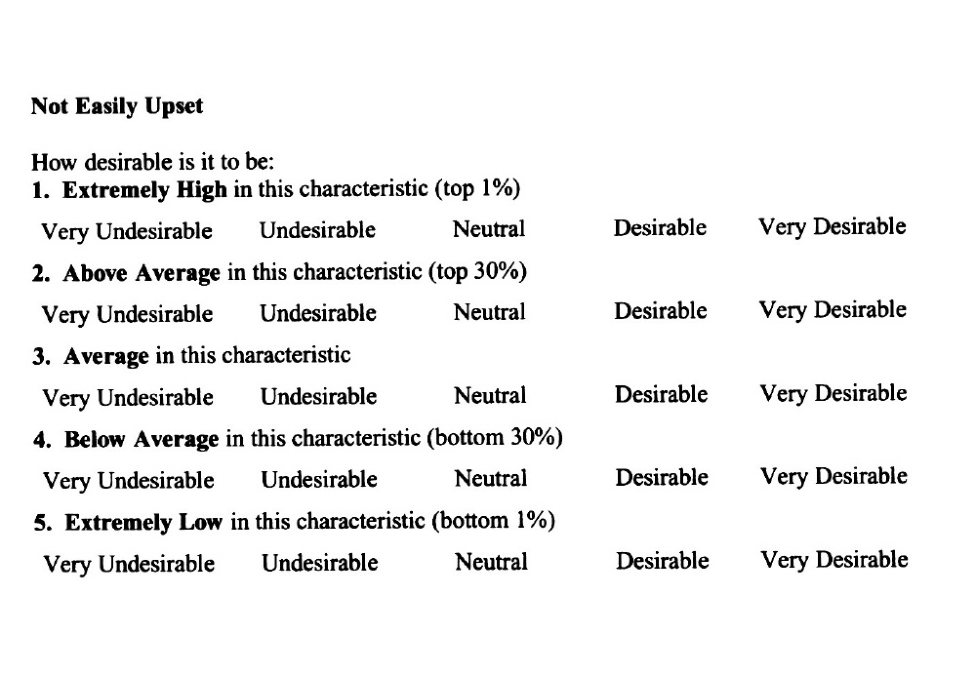
\includegraphics{KuncelTellegen_files/figure-latex/Figure1-1.pdf}
\caption{\label{fig:Figure1}Kuncel and Tellegen (2009) method for determining socially desirable saturation at the item response level.}
\end{figure}

Although there is both theoretical and empirical support for Kuncel and Tellegen (2009)'s procedure, it also quite substantially more time- and (we propose) effort-intensive than is the traditional item-rating approach (Edwards, 1953, e.g., 1957b). As technically specified, the \emph{traditional} Edwards procedure requires one evaluation per item (albeit that evaluation is made across nine levels of social desirability). The \emph{contemporary} ``Kuncel and Tellegen'' procedure requires (with common 5-point Likert-type indicators) five evaluations across five levels of desirability per item. In addition to the greater \emph{number} of evaluations required in the contemporary approach (requiring a longer time commitment from item judges), we propose that the contemporary approach is also likely more cognitively demanding due to shifting frames of reference (the referent of appraisal is variable across ratings).

\begin{quote}
Possibly integrate shifting \& cognitive load here. Kulas tried a search to no avail - Melcher suggested searching for ``perspective shift'' (5/10/21)
\end{quote}

Given the greater time and (we argue) resource commitments required of the contemporary approach (relative to the traditional), we aim to gauge to what extent these two approaches in fact capture similar versus unique pieces of information. The goal of the present investigation is therefore to directly compare these two methodologies with an ``additional information'' orientation - that is, is the new approach truly unique, or rather does it at least with some indicators convey somewhat redundant information as the classic, cognitively easier and less time-intensive approach?

\hypertarget{study-1}{%
\section{Study 1}\label{study-1}}

\hypertarget{methods}{%
\section{Methods}\label{methods}}

\hypertarget{participants}{%
\subsection{Participants}\label{participants}}

Seventy-six undergraduate students made ratings of \emph{either} item social desirability (\emph{n} = 14) (Edwards, 1957b), or levels of desirability associated with different trait levels (\emph{n} = 62; (e.g., Kuncel \& Tellegen, 2009)).

\hypertarget{materials}{%
\subsection{Materials}\label{materials}}

The IPIP-NEO is a 300-item personality measure intended to assess the Big Five personality dimensions: Conscientiousness, Agreeableness, Extraversion, Openness to Experience, and Neuroticism (Johnson, 2005). For the purposes of the current investigation, we did not collect typical responses to these 300 indicators, but were rather interested in the nature of the items themselves (or, alternatively, the evaluative content associated with differential standing along the construct implied by the item response options).

\hypertarget{procedure}{%
\subsection{Procedure}\label{procedure}}

All ratings were made via paper and pencil in an experimental laboratory. The Edwards (1957b) ratings were made along Edwards' originally specified 9-point scale ranging from (-4) Extremely Undesirable to (+4) Extremely Desirable. Because we investigated a fairly large instrument, we constructed 2 counterbalanced ``Edwards'' forms as an effort to limit potential fatigue effects across the rating process. The Kuncel and Tellegen (2009) ratings were collected from 60 different item stems across 10 different counterbalancings. Each rater (regardless of task - item stem or response option rating) was therefore asked to perform 300 total ratings (either 1 rating per 300 items or 5 ratings per 60 items).

\hypertarget{results}{%
\section{Results}\label{results}}

All analyses were performed in R version 4.1.1 (R Core Team, 2021). We leveraged three different approaches comparing findings across the two item rating procedures. First, we fit linear regressions to all ``Kuncel \& Tellegen'' functions (as explained below), focusing on the slopes, then regressed Edwards' ratings on slope coefficients across items. Secondly, we collected visual estimates of the monotonicity and linearity of these functions, and used these estimates to help inform ranges of Edwards values along which nonlinear item functions tend to be more prominent (e.g., how many ``inverted U-shaped'' functions were noted in items characterized by Edwards' system as \emph{extremely undesirable}, \emph{undesirable}, \emph{average}, \emph{desirable}, and \emph{extremely desirable}). Lastly, we conducted 300 hierarchical polynomial regressions to capture ``U'' or ``inverted-U'' functional forms, and tallied how many items were incrementally characterized by a quadratic (``above and beyond'' the linear) equation.\footnote{Note that two of these analyses share some inellegance due to a categorization of Edwards' values (e.g., there are ranges of values within each of these 5 categories; see, for example, Cohen, 1983) - we chose to categorize within crude strata because such oversimplification \emph{does} quite dramatically facilitate the communication of these results.}

For the first investigative approach (linearity of function across ``Kuncel and Tellegen'' values) several regressions were fit using the five different rated trait locations as predictors (e.g., Kuncel and Tellegen (2009)'s ``bottom 1\%,'' ``bottom 30\%,'' ``Average,'' ``top 30\%,'' and ``top 1\%'' - these were treated as an ordinal continuum {[}1, 2, 3, 4, and 5{]}) and averaged response desirability rating as the criterion (see Figure 2 for exposition - regressions were fit to the plotted space {[}response category on the x-axis and average rating on the y-axis{]}). For example, the expectation was that Figure 2's ``Excel in what I do'' and ``Believe that others have good intentions'' would realize negative slope estimates, ``Enjoy wild flights of fancy'' would exhibit a flat slope, and ``Get irritated easily'' would return a moderately positive slope. Within each of the 300 regressions, the expectation was that slope magnitude and valence would parallel the classic Edwards ratings of the same items

In order to capture the extremity of function across Kuncel and Tellegen (2009) values, several regressions\footnote{Polynomial regressions were also conducted to capture functional form but are not presented as a central index - these are however available from the authors upon request (indeed this manuscript was generated via the \texttt{R} package \texttt{papaja} (Aust \& Barth, 2021) and consistent with reproducible research standards the entire self-contained project is available upon request).} were fit using trait location as a predictor (e.g., Kuncel and Tellegen (2009)'s ``Lower 1\%,'' ``Lower 30\%,'' ``Median,'' ``Upper 30\%,'' and ``Upper 1\%'' were treated as a scaled continuum) and average desirability rating as the criterion. Slopes were retained for each function, with the expectation that slope magnitude and valence would parallel the classic Edwards ratings.

Across all 300 items, the relationship was strong (\emph{R2} = .67, \emph{p} \textless{} .05), suggesting some level of similarity across procedures. Figure 3 demonstrates these relationships for 25 randomly selected items within five categorized Edwards arrays. Note that the functions (even if somewhat non-monotonic - see, for example, ``Seldom Daydream'' in Figure 3) tend to exhibit greater slope Edwards' highly desirable or undesirable items, and are ``flatter'' with Edwards' moderate items.

Next, functional slopes of the 300 items (e.g., the Figure 2 plots for all 300 items) were rated along dimensions of ``on the whole, this looks like a straight line'' with possible ratings ranging from (1 = not at all, to 5 = definitely), and how much the ``line rises and falls'' from (1 = not at all, to 5 = a lot). These estimates were added to the first approach (defining each Edwards/Kuncel and Tellegen convergence with ratings of both functional linearity and monotonicity) and the result is presented in Figure 4. Careful inspection of the Figure 4 plot again highlights the location of non-monotonic and nonlinear Kuncel and Tellegen functions - predominantly at moderate (around neutral) Edwards rating locations.

Our third approach leveraged hierarchical polynomial regressions, with our index of interest being the change in \emph{R2} at the second step, when the polynomial terms were specified. Most items (\emph{n} = 203) had a very low change in \emph{R2} (see Table 1 for a summary of these results and a specification of our definition of ``low'' or ``very low''). Beyond our subjective categorization, \emph{F}-tests indicated that 92.31\% of item ratings were \emph{not} significantly predicted when specifying the quadratic term, and only 7.69\% were.

\hypertarget{discussion}{%
\section{Discussion}\label{discussion}}

Across approaches, results tended to converge on similar conclusions. The preponderance of our results first suggest that, in general (at least with our focal 300-item measure), linear relationships with social desirability (across response options) may be commonplace and in fact fairly well represent the plurarity of assessment item functions. Additionally, similar information seems to be available through both the traditional and contemporary measurement approaches. Although non-monotonic functions do exist, they are predominantly associated with moderately rated Edwards items. Cursory review of our randomly sampled 25 items (Figure 3) would agree with this conclusion. It is quite plausible that ``U'' or ``inverted U'' shaped functions, when they occur, are reflective of some ambiguous or contextually primed desirability, and that this ambiguity or contextual moderation results in ``middle ground'' evaluation via the Edwards method.

Undoubtedly, the Kuncel and Tellegen (2009) procedure conveys information not contained in the classic Edwards (1957b) approach. The purpose of this investigation, however, was to document overlap between the two procedures. While it is clear nonmonotonic functions do exist for some indicators across scaled ``trait levels,'' the vast majority of such circumstances are located within a range what the Edwards (1957b) procedure labels as merely moderately desirable or undesirable. There is surely additional information contained within these items, but the current investigation suggests that perhaps the more cognitively taxing and time-intensive procedure should be retained only for the items first identified by the cognitively-easier and less time-consuming Edwards (1957b) method. Our recommendation is to therefore retain both procedures, utilizing the cognitively easier and less time-consuming procedure as an initial evaluation and following-up with moderately desirable items to probe for more complex relationships.

\hypertarget{results-1}{%
\section{Results}\label{results-1}}

\textbf{THIS SECTION IS ALSO NOT IN THE PAPER, BUT DID NOT WANT TO DELETE EVERYTHING WITHOUT PERMISSION}

The plurality of findings do support similar infomration being conveyed through both approaches. Figure 1 captures \emph{some} of this, as functional slopes (even if somewhat nonmonotonic - see, for example, ``Seldom Daydream'' in Figure 1) tend to be more extreme with Edwards' highly desirable or undesirable items, and more flat with Edwards' moderate items.\footnote{These items were randomly sampled from within Edwards-rating strata. Visuals of all items' functional forms are available from the authors upon request.} Table 1 presents the frequency with which researcher-implicated functional shapes (linear {[}positive{]}, linear {[}negative{]}, nonmonotonic {[}U{]}, and nonmonotonic {[}inverted U{]}) were noted within ``Edwardian'' strata, demonstrating that although the nonmonotonic functions do exist, they are predominantly associated with moderate Edwards items (e.g., yes these functions do occur but perhaps the ambivalence is also associated with aggregate moderation). Figure 2 presents the relationship between: 1) the functional slope relating an item response's rated level of desirability and the ``location'' of the rating, and 2) Edwards' item stem rating (on the y-axis). This strong relationship (\emph{R}\^{}2 = .67, \emph{p} \textless{} .05) suggests some level of similarity across procedures.

\hypertarget{study-two}{%
\section{Study Two}\label{study-two}}

\begin{quote}
put in some references regarding response latencies
\end{quote}

One of our observations across the two item rating procedures has been that the Kuncel and Tellegen (2009) approach appears to be more cognitively taxing for ``raters'' than does the Edwards (1953). Study Two therefore collected ratings via computer, with response latencies recorded as well as direct self-reported estimates of difficulty. The same indicators were retained for Study Two.

\hypertarget{procedure-1}{%
\subsection{Procedure}\label{procedure-1}}

The Study One items were administered via Qualtrics (2014). Participants were administered directions for each condition: 1) Edwards rating, 2) Kuncel \& Tellegen rating, and 3) modified Kuncel \& Tellegen rating. This third condition was included as a possible compromise to the \emph{anticipated} cognitive difficulty associated with the Kuncel \& Tellegen procedure. Here, we ask participants to focus on only one of the Kuncel \& Tellegen ``levels'' (e.g., across items, the rating category is held constant). We coded items for length and presence of a ``negative'' qualifier (e.g., I would never lie). Anecdotally, the presence of a negative element within an item stem contributed to difficulty for raters.

In addition to actual ratings, we also recorded latencies, which we interpret as indirect assessments of difficulty.

Because of the tedium and cognitive complexity of the requested task, we computed consecutive non-differentiating responses as well as intra-individual response variability estimates (see, for example, Dunn, Heggestad, Shanock, \& Theilgard, 2018; Marjanovic, Holden, Struthers, Cribbie, \& Greenglass, 2015) via the \emph{careless} R package (Yentes \& Wilhelm, 2021) in R version 4.1.1 (R Core Team, 2021).

Table to add: ICC's for each condition

Focus on response latencies (Edwards ratings vs.~Kuncel \& Tellegen vs.~revised Kuncel \& Tellegen (split by rated category). Indices here are: 1) response latencies, 2) inter-rater agreement/reliability\footnote{NOTE TO SELVES - WHEN WE DO THE SECOND PART (RESPONSE LATENCIES), MAKE SURE TO CODE NEGATIVELY-WORDED STEMS (THESE SEEM ESPECIALLY DIFFICULT TO RATE USING THE KUNCEL \& TELLEGEN PROCEDURE)}

\hypertarget{results-2}{%
\section{Results}\label{results-2}}

\begin{figure}
\centering
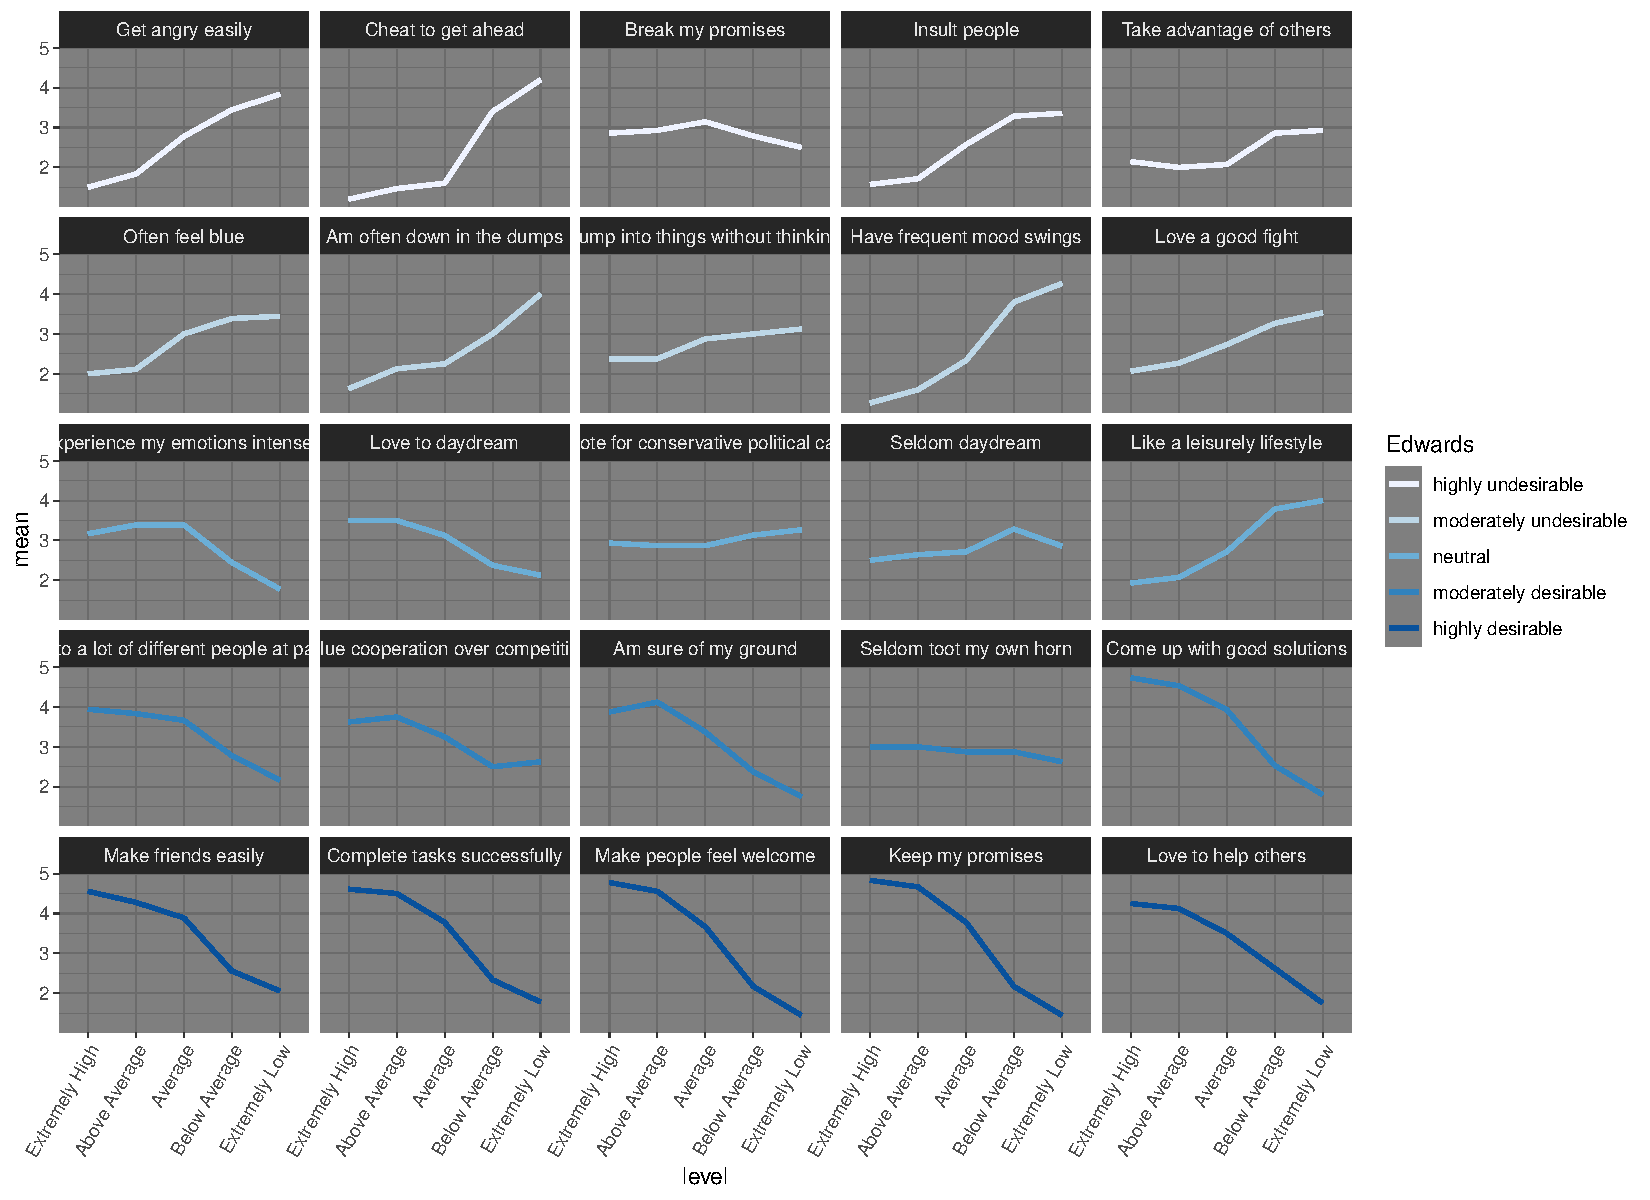
\includegraphics{KuncelTellegen_files/figure-latex/Figure2-1.pdf}
\caption{\label{fig:Figure2}Kuncel \& Tellegen (2009) patterns across Edwards (1953) scale values.}
\end{figure}

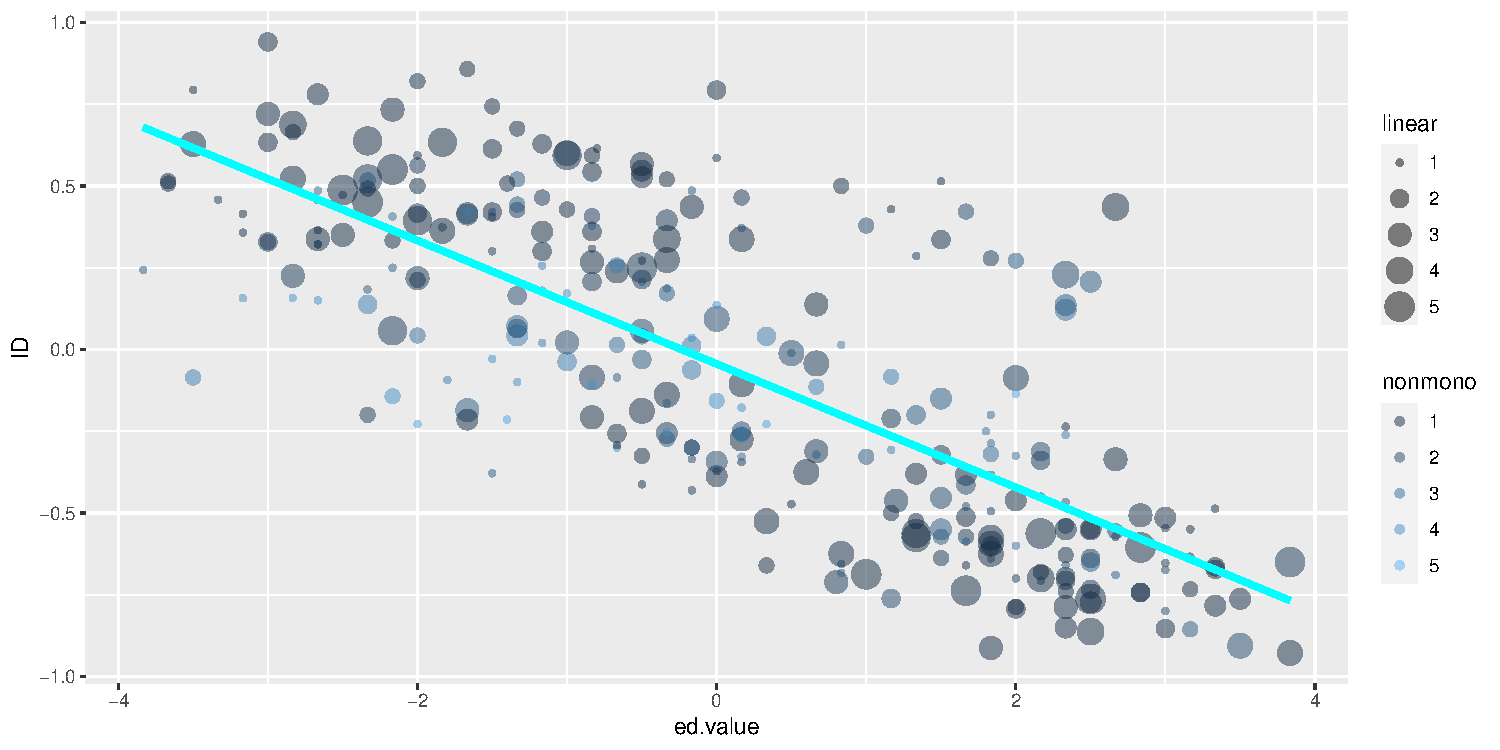
\includegraphics{KuncelTellegen_files/figure-latex/Figure3-1.pdf}
The intercept was -3.08 \textless- just testing.

\hypertarget{discussion-1}{%
\section{Discussion}\label{discussion-1}}

Certainly the Kuncel and Tellegen (2009) procedure conveys information not contained in the classic Edwards (1957b) approach. The purpose of this investigation, however, was to document overlap between the two procedures. Clearly nonmonotonic functions do exist for some indicators across scaled ``trait levels.'' However, the vast majority of such circumstances are located within what the Edwards (1957b) procedure labels as ``moderately desirable.'' There is certainly additional information contained within these items, but the current investigation suggests that perhaps the more cognitively taxing and time-intensive procedure be retained for only those items first identified by the cognitively-easier and less time consuming Edwards (1957b) method as ``moderately desirable.''

\hypertarget{limitations}{%
\subsection{Limitations}\label{limitations}}

Our task was likely too long - in retrospect a shorter measure should have been pursued.

\hypertarget{references}{%
\section{References}\label{references}}

\begingroup
\setlength{\parindent}{-0.5in}
\setlength{\leftskip}{0.5in}

\hypertarget{refs}{}
\begin{CSLReferences}{1}{0}
\leavevmode\hypertarget{ref-alicke_self-enhancement_2009}{}%
Alicke, M. D., \& Sedikides, C. (2009). Self-enhancement and self-protection: What they are and what they do. \emph{European Review of Social Psychology}, \emph{20}(1), 1--48.

\leavevmode\hypertarget{ref-alicke_handbook_2011}{}%
Alicke, M. D., \& Sedikides, C. (2011). \emph{Handbook of self-enhancement and self-protection}. Guilford Press.

\leavevmode\hypertarget{ref-R-papaja}{}%
Aust, F., \& Barth, M. (2021). \emph{Papaja: Prepare reproducible APA journal articles with r markdown}. Retrieved from \url{https://github.com/crsh/papaja}

\leavevmode\hypertarget{ref-barrick_what_2009}{}%
Barrick, M. R., Shaffer, J. A., \& DeGrassi, S. W. (2009). What you see may not be what you get: Relationships among self-presentation tactics and ratings of interview and job performance. \emph{Journal of Applied Psychology}, \emph{94}(6), 1394.

\leavevmode\hypertarget{ref-birkeland_meta-analytic_2006}{}%
Birkeland, S. A., Manson, T. M., Kisamore, J. L., Brannick, M. T., \& Smith, M. A. (2006). A meta-analytic investigation of job applicant faking on personality measures. \emph{International Journal of Selection and Assessment}, \emph{14}(4), 317--335.

\leavevmode\hypertarget{ref-cohen_cost_1983}{}%
Cohen, J. (1983). The cost of dichotomization. \emph{Applied Psychological Measurement}, \emph{7}(3), 249--253.

\leavevmode\hypertarget{ref-crowne_new_1960}{}%
Crowne, D. P., \& Marlowe, D. (1960). A new scale of social desirability independent of psychopathology. \emph{Journal of Consulting Psychology}, \emph{24}(4), 349.

\leavevmode\hypertarget{ref-dauenheimer_self-enhancement_2002}{}%
Dauenheimer, D. G., Stahlberg, D., Spreemann, S., \& Sedikides, C. (2002). Self-enhancement, self-verification, or self-assessment? The intricate role of trait modifiability in the self-evaluation process. \emph{Revue Internationale de Psychologie Sociale}.

\leavevmode\hypertarget{ref-dimoulas_patterns_1998}{}%
Dimoulas, E., Wender, S., Keenan, J. P., Gallup, G., \& Goulet, N. (1998). Patterns of deception in human mating strategies. \emph{Journal of Psychology and the Behavioral Sciences}, \emph{12}, 39--42.

\leavevmode\hypertarget{ref-donovan_impact_2014}{}%
Donovan, J. J., Dwight, S. A., \& Schneider, D. (2014). The impact of applicant faking on selection measures, hiring decisions, and employee performance. \emph{Journal of Business and Psychology}, \emph{29}(3), 479--493.

\leavevmode\hypertarget{ref-dunn_intra-individual_2018}{}%
Dunn, A. M., Heggestad, E. D., Shanock, L. R., \& Theilgard, N. (2018). Intra-individual response variability as an indicator of insufficient effort responding: Comparison to other indicators and relationships with individual differences. \emph{Journal of Business and Psychology}, \emph{33}(1), 105--121.

\leavevmode\hypertarget{ref-edwards_relationship_1953}{}%
Edwards, A. L. (1953). The relationship between the judged desirability of a trait and the probability that the trait will be endorsed. \emph{Journal of Applied Psychology}, \emph{37}(2), 90--93.

\leavevmode\hypertarget{ref-edwards_social_1957-4}{}%
Edwards, A. L. (1957a). Social desirability and probability of endorsement of items in the interpersonal check list. \emph{The Journal of Abnormal and Social Psychology}, \emph{55}(3), 394--396.

\leavevmode\hypertarget{ref-edwards_social_1957}{}%
Edwards, A. L. (1957b). \emph{The social desirability variable in personality assessment and research.} Ft Worth, TX, US: Dryden Press.

\leavevmode\hypertarget{ref-kuncel_conceptual_2009}{}%
Kuncel, N. R., \& Tellegen, A. (2009). A conceptual and empirical reexamination of the measurement of the social desirability of items: Implications for detecting desirable response style and scale development. \emph{Personnel Psychology}, \emph{62}(2), 201--228.

\leavevmode\hypertarget{ref-leising_vocabulary_2012}{}%
Leising, D., Ostrovski, O., \& Borkenau, P. (2012). Vocabulary for describing disliked persons is more differentiated than vocabulary for describing liked persons. \emph{Journal of Research in Personality}, \emph{46}(4), 393--396.

\leavevmode\hypertarget{ref-leising_model_2015}{}%
Leising, D., Scherbaum, S., Locke, K. D., \& Zimmermann, J. (2015). A model of {``substance''} and {``evaluation''} in person judgments. \emph{Journal of Research in Personality}, \emph{57}(1), 61--71.

\leavevmode\hypertarget{ref-levashina_model_2006}{}%
Levashina, J., \& Campion, M. A. (2006). A model of faking likelihood in the employment interview. \emph{International Journal of Selection and Assessment}, \emph{14}(4), 299--316.

\leavevmode\hypertarget{ref-li_using_2006}{}%
Li, A., \& Bagger, J. (2006). Using the {BIDR} to distinguish the effects of impression management and self-deception on the criterion validity of personality measures: A meta-analysis. \emph{International Journal of Selection and Assessment}, \emph{14}(2), 131--141.

\leavevmode\hypertarget{ref-marjanovic_inter-item_2015}{}%
Marjanovic, Z., Holden, R., Struthers, W., Cribbie, R., \& Greenglass, E. (2015). The inter-item standard deviation ({ISD}): An index that discriminates between conscientious and random responders. \emph{Personality and Individual Differences}, \emph{84}, 79--83.

\leavevmode\hypertarget{ref-morgeson_reconsidering_2007}{}%
Morgeson, F. P., Campion, M. A., Dipboye, R. L., Hollenbeck, J. R., Murphy, K., \& Schmitt, N. (2007). Reconsidering the use of personality tests in personnel selection contexts. \emph{Personnel Psychology}, \emph{60}(3), 683--729.

\leavevmode\hypertarget{ref-ones_role_1996}{}%
Ones, D. S., Viswesvaran, C., \& Reiss, A. D. (1996). Role of social desirability in personality testing for personnel selection: The red herring. \emph{Journal of Applied Psychology}, \emph{81}(6), 660.

\leavevmode\hypertarget{ref-paulhus_balanced_1988}{}%
Paulhus, D. L. (1988). Balanced inventory of desirable responding ({BIDR}). \emph{Acceptance and Commitment Therapy. Measures Package}, \emph{41}, 79586--79587.

\leavevmode\hypertarget{ref-qualtrics_qualtrics_2014}{}%
Qualtrics, L. L. C. (2014). Qualtrics {[}software{]}. \emph{Utah, {USA}: Qualtrics}.

\leavevmode\hypertarget{ref-R-base}{}%
R Core Team. (2021). \emph{R: A language and environment for statistical computing}. Vienna, Austria: R Foundation for Statistical Computing. Retrieved from \url{https://www.R-project.org/}

\leavevmode\hypertarget{ref-sedikides_self-enhancement_2012}{}%
Sedikides, C., \& Alicke, M. D. (2012). \emph{Self-enhancement and self-protection motives}. Oxford handbook of motivation, ed. R. Ryan. Oxford University Press.{[}{rWvH}{]}.

\leavevmode\hypertarget{ref-taylor_illusion_1988}{}%
Taylor, S. E., \& Brown, J. D. (1988). Illusion and well-being: A social psychological perspective on mental health. \emph{Psychological Bulletin}, \emph{103}(2), 193.

\leavevmode\hypertarget{ref-viswesvaran_meta-analyses_1999}{}%
Viswesvaran, C., \& Ones, D. S. (1999). Meta-analyses of fakability estimates: Implications for personality measurement. \emph{Educational and Psychological Measurement}, \emph{59}(2), 197--210.

\leavevmode\hypertarget{ref-weiss_looking_2006}{}%
Weiss, B., \& Feldman, R. S. (2006). Looking good and lying to do it: Deception as an impression management strategy in job interviews. \emph{Journal of Applied Social Psychology}, \emph{36}(4), 1070--1086.

\leavevmode\hypertarget{ref-R-careless}{}%
Yentes, R., \& Wilhelm, F. (2021). \emph{Careless: Procedures for computing indices of careless responding}. Retrieved from \url{https://github.com/ryentes/careless/}

\leavevmode\hypertarget{ref-ziegler_applicant_2011}{}%
Ziegler, M. (2011). Applicant faking: A look into the black box. \emph{The Industrial and Organizational Psychologist}, \emph{49}(1), 29--36.

\end{CSLReferences}

\endgroup


\end{document}
